% small.tex
\documentclass[t]{beamer}
\usepackage{graphicx}
\usepackage{listliketab}
\usetheme[hideothersubsections]{Goettingen}
\setbeamercolor{palette primary}{bg=structure.fg!25}
\setbeamercolor{palette secondary}{bg=structure.fg!10,fg=black}
\useinnertheme{rectangles} 
\useoutertheme{infolines} 
\author[TAES]{Thomas Smith} 
\title[CM30174/CM50206]{CM30174 + CM50206\\Intelligent Agents}
\institute[Bath/CS]{East Building}
\date{December 8, 2013} 
\begin{document}


%--- the titlepage frame -------------------------%
\begin{frame}
  \titlepage
\end{frame}

%--- the presentation begins here ----------------%
\section{Overview}
\subsection{Paper Overview}
\begin{frame}[c]{Paper Overview}
	\begin{quote}
		``Towards an environment interface standard for agent platforms''
	\end{quote}
	\hfill Tristan M. Behrens, Koen V. Hindriks, J{\"u}rgen Dix\\
	\hfill {\tiny \textit{Annals of Mathematics and Artificial Intelligence} (2011), 61:261--295.}
\end{frame}
\subsection{Problem Overview}
\begin{frame}{Problem Overview}
	Issues:
	\pause
	\begin{itemize}[<+->]
		\item There are many Agent Programming Languages (\emph{APL}s)
		\begin{itemize}
			\item<3-> 2APL
			\item<3-> \textsc{Goal}
			\item<3-> \textsc{Jadex}
			\item<3-> \textit{Jason}
		\end{itemize}
		\pause
		\item Multiple varied environments are used
		\begin{itemize}
			\item<5-> Trading Agent Competition
			\item<5-> MASSim Agent Competitions
			\item<5-> Unreal Tournament 2004
		\end{itemize}
		\pause
		\item How can we connect / compare these components?
		\begin{itemize}
			\item Connections: TCP/IP, RMI, wrapping Java code, JNI
			\item Comparisons: we can't
		\end{itemize}
	\end{itemize}
\end{frame}

\subsection{Goals}
\begin{frame}{Goals}
		%Motivation
	\begin{itemize}[<+->]
		\item Implementing an environment interface standard would:\nolinebreak\begin{itemize}
			\item make already working environments widely available
			\item facilitate distribution of current and future environments
			\item allow direct comparison of APL platforms
			\item enable the development of a fully heterogeneous multi-agent system (\emph{MAS})
		\end{itemize}
		% \begin{quote}
		% 	Lessons learned have not been documented well enough to enable transfer of knowledge in this area
		% \end{quote}
		%Requirements
		\item In order to be accepted as a standard, it should:
		\begin{itemize}
			\item Provide an interface that is as \textit{generic as possible}
			\item \textit{Reuse as much as possible} from existing interfaces
			%obvious trade-off here
		\end{itemize}
		\item Therefore the objective is to: 
		\begin{itemize}
			\item[] \ 
			\item[]<10->``\textit{Design and develop an environment interface standard (\emph{EIS}) that facilitates connecting agents programmed in various agent platforms to environments.}''
		\end{itemize}
	\end{itemize}
\end{frame}
\begin{frame}{Goals (contd.)}
	\begin{itemize}[<+->]
		\item Ideally, no assumptions should be made about the internal structure or behaviour of any of the environments or entities
		\item However, the agent platform needs to support a minimal agent-based abstraction: \linebreak \textit{Actions and percepts are treated as first-class entities.}
		\item The standard is based on:
		\begin{itemize}
			\item A meta-model for agent-environment interaction
			\item A set of principles that encode useful constraints for implementing the standard
		\end{itemize}
		\item The meta-model arises from a study of existing APLs, and avoids restricting existing approaches
		\item The principles arise from the requirements of the project, and observed best practices in existing research
	\end{itemize}
\end{frame}
\begin{frame}{Principles}
	\begin{enumerate}[<+->]
		\item \textit{Portability}: .jar files are suggested but not required, for easy exchange of environments between platforms
		\item \textit{Generality}: The \emph{EIS} should impose minimal restrictions on the platform or environments. Assumptions about the agents or the environments should be avoided
		\item \textit{Separation of concerns}: Agents are \textit{separated} from the environment, agents \textit{map to} controllable entities
		\item \textit{Unified connections}: The \emph{EIS} should facilitate communications between agents and the environment(s)
		\item \textit{Standards for actions/percepts/events/etc.}: The \emph{EIS} should provide a convention for communicating about concepts, without restricting any existing approach
		\item \textit{Support for heterogeneity}: The \emph{EIS} needs to facilitate heterogeneity - connections between an environment and agents of multiple types
	\end{enumerate}
\end{frame}
\section{Existing Work}
\subsection{Related Work}
\begin{frame}{Related Work}
	There are a number of other projects that support generic connections between agents and an environment:
	\pause
	\begin{itemize}[<+->]
		\item A\&A: a generic paradigm for modelling environments. Implemented in the distributed middleware \textsc{CArtAgO}
		\item \textsc{Soar} is an architecture for knowledge-rich agents capable of intelligent behaviour in dynamic environments
		\item GameBots and Pogamut are a pair of projects designed to allow agents to control bots in UT2004. A number of other projects use them as an initial base
		\begin{itemize}
			\item pyPOSH aims to use Behaviour Oriented Design agents
			\item the ACT-R cognitive architecture uses GameBots
		\end{itemize}
		\item The high level architecture (HLA) is a federated architecture for distributed simulations
		\item The \textit{UtJackInterface} defines another UT2004 interface from scratch
	\end{itemize}
	% does not facilitate reuse
\end{frame}
\subsection{Existing APLs}
\begin{frame}{Existing Agent Programming Languages}
	\begin{itemize}[<+->]
		\item A number of existing APLs indicate common and uncommon features that the meta-model must support
		\begin{itemize}
		\item<2-> 2APL
		% Environments are distributed as jar-files. Agents can be associated with several environments, jars have to be in the user-directory. Agents are objects, there is a communications format
		\item<2-> \textsc{Goal}
		% Environments are distributed as jar-files. There is a scheduler.
		\item<2-> \textsc{Jadex}
		% Environments exist as belifs of the agents.
		\item<2-> \textit{Jason}
		% Environments are distributed as jar-files. Each MAS has at most one environment. Sophisticated abstract environments
		\end{itemize}
		\pause
		\item Though each APL is designed to fulfil similar purposes, they vary in implementation details
		\begin{itemize}
			\item 2APL provides a common format for exchanging data between agents and the environment
			\item \textsc{Goal} uses a scheduler to manage execution of agents
			\item \textsc{Jadex} store environments as beliefs of the agents
			\item \textit{Jason} provides sophisticated abstract environments
		\end{itemize}
		\item The different APLs have differing degrees of environment management functionality available
	\end{itemize}
\end{frame}
\subsection{Existing Environments}
\begin{frame}{Existing Environments}
\begin{itemize}
	\item<1-> Elevator environment
	\begin{itemize}
		\item[] The elevator environment is a simulator of arbitrary multi-elevator environments where elevators are controllable entities that agents can manage
	\end{itemize}
	\item<2-> The Trading Agent Competition
	\begin{itemize}
		\item[] The TAC is an annual competition run on a research testbed for autonomous bidding agents. The interface uses TCP/IP and is time-sensitive
	\end{itemize}
	\item<3-> MASSim
	\begin{itemize}
		\item[] The \textit{AgentContest} environment is a discrete simulation that relies on co-operation and co-ordination between multiple agents. Communication uses XML wrappers
	\end{itemize}
	\item<4-> Unreal Tournament 2004
	\begin{itemize}
		\item[] UT2004 is a popular real-time testbed for continuous, dynamic multi-agent interaction environments. High- or low-level interaction is possible
	\end{itemize}
\end{itemize}
\end{frame}
\section{EIS}
\subsection{Meta-model}
\begin{frame}{Meta-model}
	\begin{figure}
		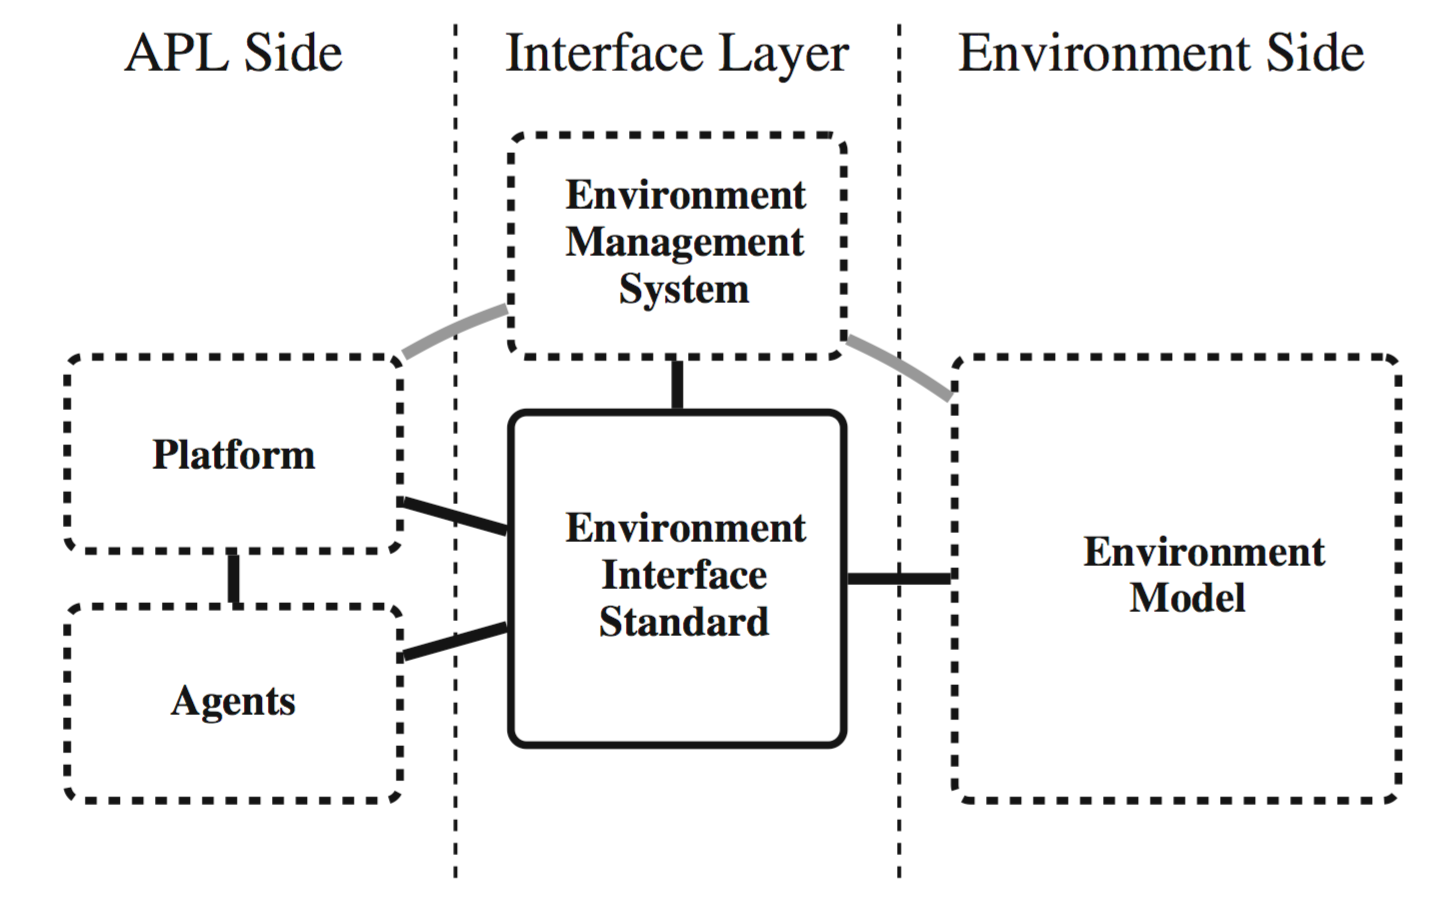
\includegraphics[width=0.6\linewidth]{metamodel}
	\end{figure}
% This model also includes generic functionality for managing an environment.
% The model introduced below is called a meta model as it does not describe a specific agent–environment interface but is intended to describe generic functionality that should be available in any agent-based interface supporting agent–environment interaction.
	\small
	\begin{enumerate}
		\item<1-> \textit{Agent}\only<1>{: able to perceive its environment through sensors and act upon that environment through effectors.}
		\item<2-> \textit{Environment model}\only<2>{: contains \textit{controllable entities} that give agents effective and sensory presence in the environment.}
		\item<3-> \textit{Platform}\only<3>{: instantiates and executes agents; connects agents to the environment and controllable entities.}
		\item<4-> \textit{Environment management system (EMS)}\only<4>{: provides actions for managing an environment, such as setup, pause and reset.}
		\item<5-> \textit{Environment interface standard (EIS)}\only<5>{: the layer that connects the platform, the EMS, and the agents to the environment(s).}
	\end{enumerate}
\end{frame}
\subsection{Interface Immediate Language}
\begin{frame}{Interface Immediate Language}
\begin{itemize}[<+->]
	\item The interface immediate language (\emph{IIL}) facilitates the exchange of data between different components
	\item It provides an implementation-agnostic method for communicating about percepts, actions, and events
	\item The language consists of:
	\begin{itemize}
		\item \textit{Data containers}, which represent \textit{actions} performed by agents, \textit{results} of actions, and \textit{percepts}. There are also \textit{environment commands} that control the execution of the environment
		\item Data container \textit{parameters}, which are either constant numerals and identifiers or functions over (lists of) parameters
	\end{itemize}
	\item Example server connection code:\nolinebreak\begin{itemize}
		\item[]<6-> \texttt{action(connect,agentsim1,team1,pa55w0rd)}
	\end{itemize}
\end{itemize}
\end{frame}
\subsection{Implementation}
\begin{frame}{Implementation}
\begin{itemize}[<+->]
	\item Two-way connections are provided via interactions performed by the components and notifications performed by the \emph{EIS}
	\begin{itemize}
		\item Interactions are (possibly remote) function calls to the \emph{EIS}, that can return a value
		\item Notifications follow the observer design pattern, components are \textit{listeners} that have callback functions
	\end{itemize}
	\item For agents, the two methods correspond to the notions of \textit{polling} and \textit{interrupts}
	\item Agents exist on the platform side, controllable entities exist in the environment, and agents may control entities through the \emph{EIS} mapping between sets
	\item The \emph{EIS} manages the sets of entities and agents, the mapping, observer notifications, and controlling manageable aspect of the environment
\end{itemize}
\end{frame}
\section{Case Studies}
\subsection{Case Study: Elevator}
\begin{frame}{Case Study: Elevator}
	\begin{figure}
		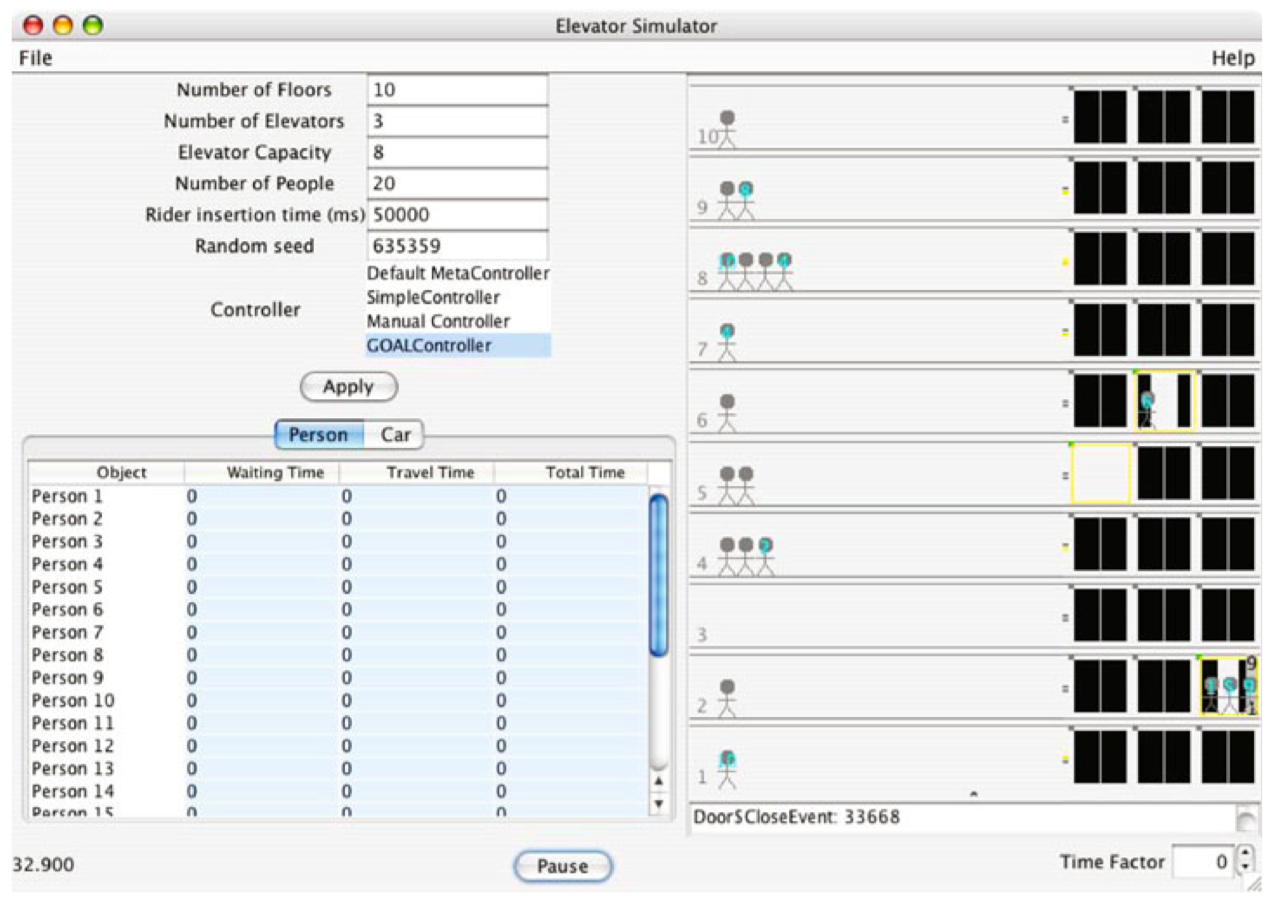
\includegraphics[width=0.9\linewidth]{elevator}
	\end{figure}
\end{frame}
\begin{frame}[noframenumbering]{Case Study: Elevator}
	\begin{figure}
		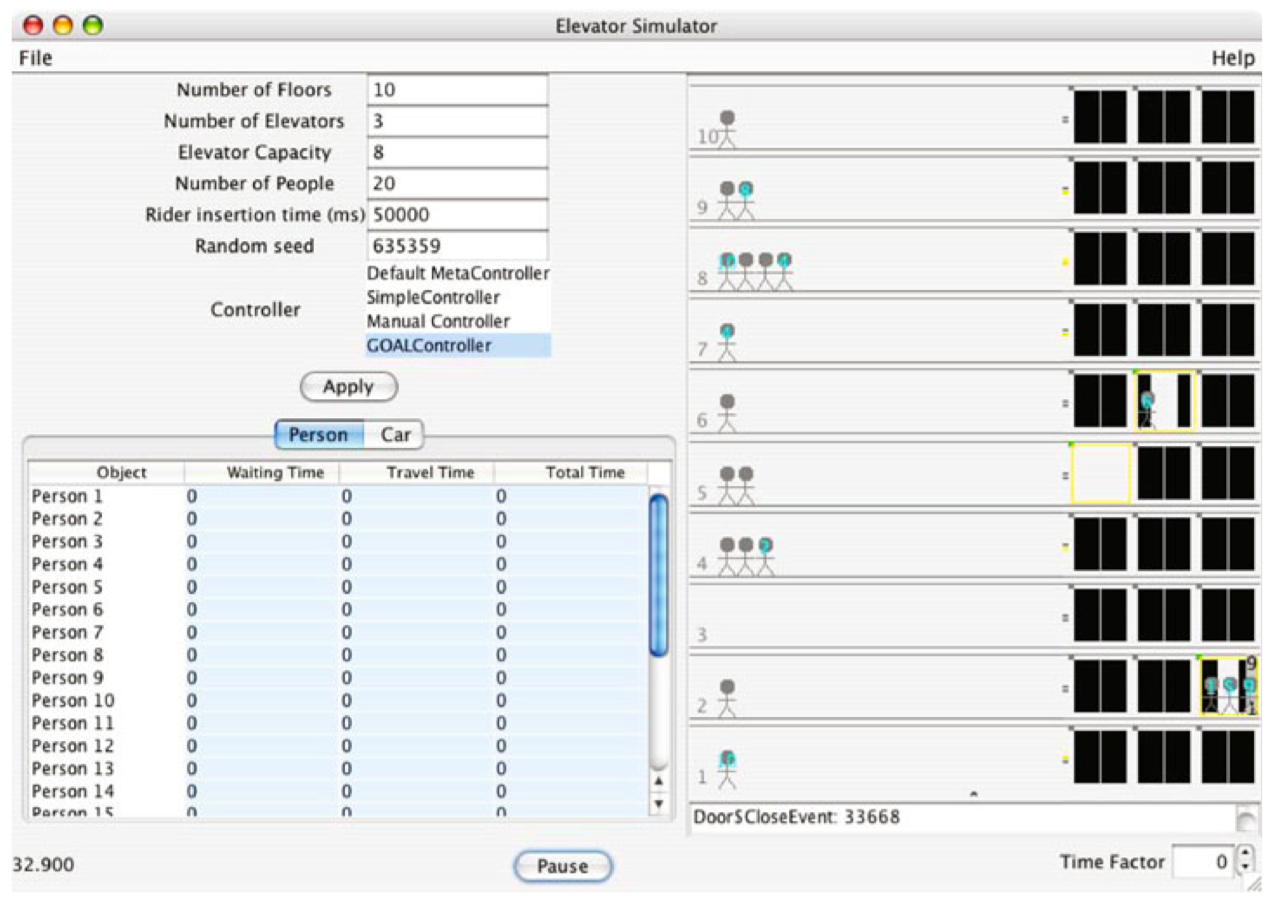
\includegraphics[width=0.55\linewidth]{elevator}
	\end{figure}
	\begin{itemize}[<+->]
		\item Not designed for agents, originally adapted for \textsc{Goal}
		\item \emph{EIS} easily handles unique aspects of the environment
		\begin{itemize}
			\item \textit{Durative actions} take time to fulfil rather than being discrete single events
			\item \emph{EIS} supports the \textit{partially observable} environment
		\end{itemize}
		\item The elevator environment can now run with 2APL, \textsc{Goal}-through-\emph{EIS}, and \textit{Jason}
	\end{itemize}
\end{frame}
\subsection{Case Study: Agent Contest}
\begin{frame}{Case Study: Agent Contest}
	\begin{figure}
		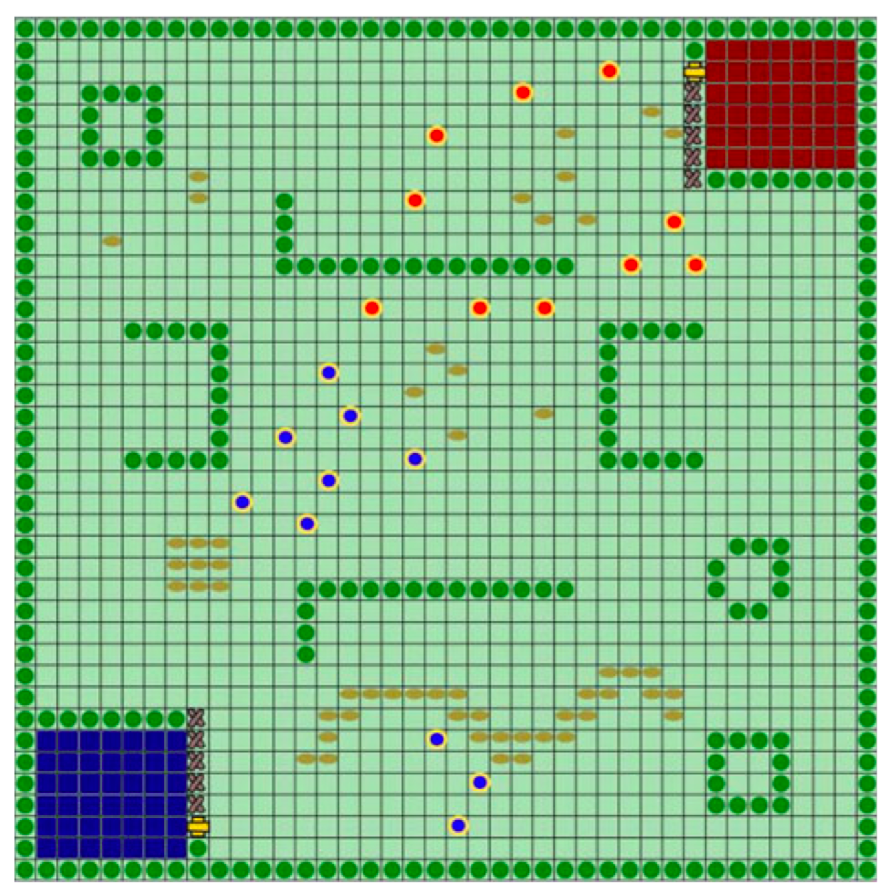
\includegraphics[width=0.7\linewidth]{cowboys}
	\end{figure}
\end{frame}
\begin{frame}[noframenumbering]{Case Study: Agent Contest}
	\begin{figure}
		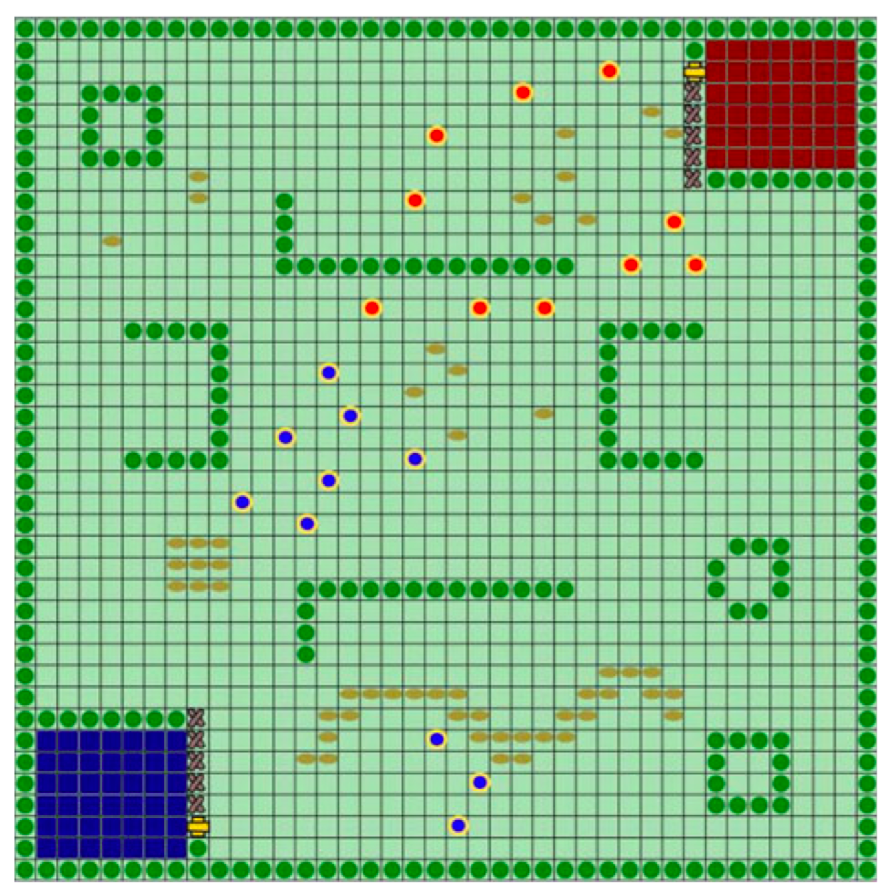
\includegraphics[width=0.45\linewidth]{cowboys}
	\end{figure}
	\begin{itemize}[<+->]
		\item Connection via TCP/IP is easily supported by the \emph{EIS}
		\item Mappings from XML to the IIL work once completed
		\item The \emph{EIS} does not impose restrictions on the connection between itself and environments
	\end{itemize}
\end{frame}
\subsection{Case Study: Unreal Tournament}
\begin{frame}{Case Study: Unreal Tournament}
	\begin{figure}
		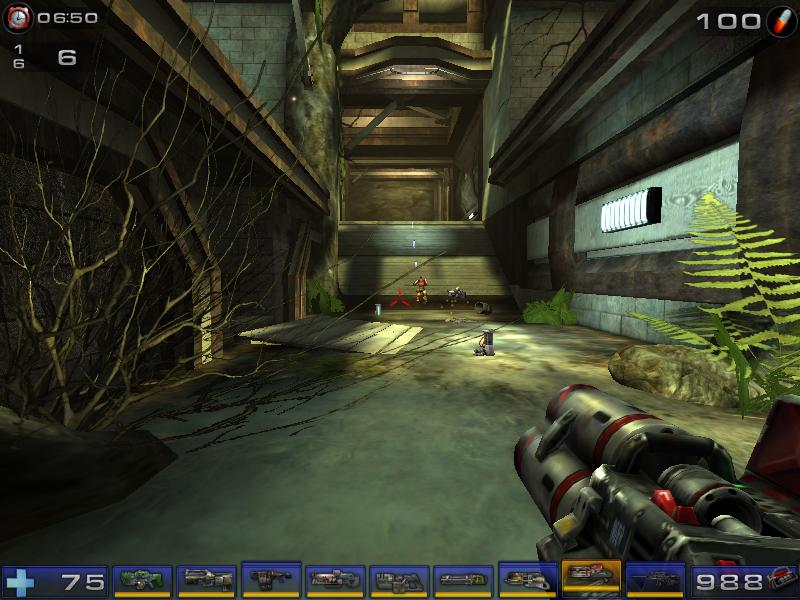
\includegraphics[width=0.95\linewidth]{ut2004}
	\end{figure}
\end{frame}
\begin{frame}[noframenumbering]{Case Study: Unreal Tournament}
	\begin{figure}
		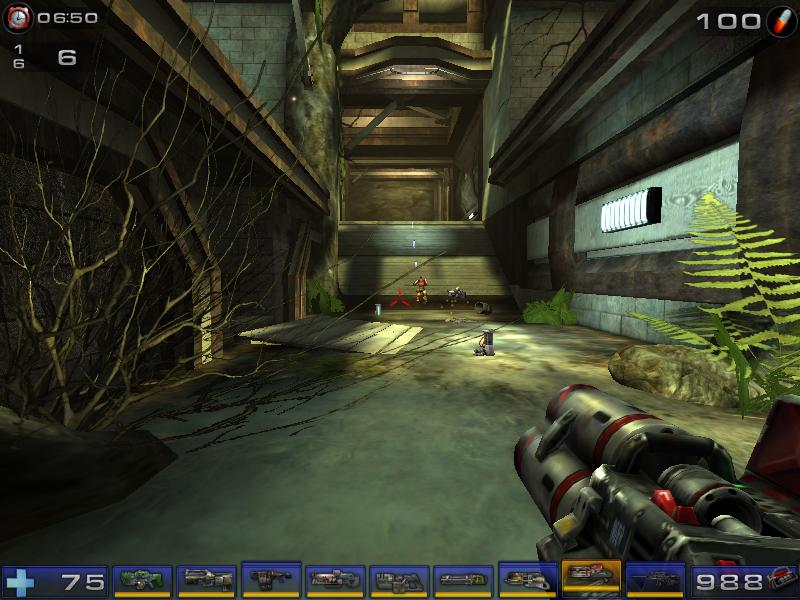
\includegraphics[width=0.6\linewidth]{ut2004}
	\end{figure}
	\begin{itemize}[<+->]
		\item More challenging due to the real-time low-level interface
		\item Interface built on \textit{Pogamut} and \textit{GameBots}
		\item Provides abstraction for high-level actions
		\item \textit{Durative actions} and delegation implemented
	\end{itemize}
\end{frame}
\section{Summary}
\begin{frame}{Summary}
	\begin{itemize}[<+->]
		\item The environment interface standard as implemented conforms to the original goals and requirements
		\item The ease with which it integrates with existing environments suggests that it supports a correct level of abstraction for agent-environment interaction
		\item It provides a number of benefits to future projects that support the interface:
		\begin{itemize}
			\item Standard functionality is provided by the interface implementation itself
			\item Agent platforms that support the interface can connect to any environment that implements the interface
		\end{itemize}
		\item The \emph{EIS} facilitates a new approach to comparison between APLs through a truly heterogeneous MAS
	\end{itemize}
\end{frame}
% \section{}
% \begin{frame}{Glossary}
% \end{frame}

\end{document}